\documentclass[conference]{IEEEtran}

\ifCLASSINFOpdf

\else

\fi


\usepackage{graphicx}
\usepackage{textcomp}
\usepackage{mathtools}
\usepackage[acronym]{glossaries}
\usepackage[backend=bibtex, style=ieee]{biblatex}
\usepackage{tabularx, caption}

\addbibresource{bibliography}
% decomment below to reduce bib font size
% \renewcommand*{\bibfont}{\small}

% acronyms
\newacronym[plural=EAs, firstplural=Evolutionary Algorithms (EAs)]{ea}{EA}{Evolutionary Algorithm}
\newacronym{er}{ER}{Evolutionary Robotics}
\newacronym[plural=NNs, firstplural=Neural Networks]{nn}{NN}{Neural Network}
\newacronym[plural=ANNs, firstplural=Artificial Neural Networks]{ann}{ANN}{Artificial Neural Network}
\newacronym{tweann}{TWEANN}{Topology \& Weight Evolving Artificial Neural Network}
\newacronym{neat}{NEAT}{NeuroEvolution of Augmenting Topologies}


% correct bad hyphenation here
\hyphenation{op-tical net-works semi-conduc-tor}


% tables config
\renewcommand{\arraystretch}{2.4}
\newcolumntype{L}[1]{>{\hsize=#1\hsize\raggedright\arraybackslash}X}%
\newcolumntype{R}[1]{>{\hsize=#1\hsize\raggedleft\arraybackslash}X}%
\newcolumntype{C}[1]{>{\hsize=#1\hsize\centering\arraybackslash}X}%


\begin{document}
 
\title{Competitive co-evolution in robots: \\ heterogeneity vs homogeneity}



\author{\IEEEauthorblockN{Selene Baez Santamaria, Andrea Jemmett, Tommie Kerstens, Enrico Rotundo}
\IEEEauthorblockA{
Vrije Universiteit Amsterdam \\
Amsterdam, Netherlands}}



\maketitle


\begin{abstract}
In the context of robotics, intelligent behaviours are often achieved using neural networks as controllers evolved using  an evolutionary algorithm.
In the case of multiple individuals within a species, controllers can be either homogeneous or heterogeneous.
In this paper, we use competitive co-evolution of homogeneous and heterogeneous controllers in order to investigate its effects on the effectiveness regarding a herding task.
Our experiments show that shepherds perform better when assigned homogeneous controllers than heterogeneous controllers.
Furthermore, we also find that task complexity is not sufficient to determine the effectiveness heterogeneous controllers have in a herding task.
\end{abstract}


\IEEEpeerreviewmaketitle


\section{Introduction}
% Evolutionary Algorithms
\glspl{ea} are biology inspired algorithms that, going through multiple steps (reproduction, mutation, recombination and selection), are able to evolve entities over time.
Thus, the entities subject to the evolution are referred to as individuals and represent candidate solutions to an optimization problem.
An \gls{ea} measures the quality of individuals using a \textit{fitness function} and its aim is to improve individuals' fitness score along successive generations.
\gls{er} is a technique that uses \gls{ea}s to develop a policy for an autonomous robot.
Its main objective is to evolve intelligent robots behaviours required to solve some real-word task.
\gls{er} implementations often rely on an \gls{ann} to represent their controllers.
% Neural Networks
An \gls{ann}, commonly referred to as \gls{nn} in this field, is a function estimator that can be used as a policy for an autonomous agent and its design is natural inspired by the biological nervous system.
In order to employ it as a controller, inputs usually come from sensors making observations of the environment and the output is then used to control an actuation schema.
The evaluation of the individuals' controllers can be made in a simulation.
This exploits the computer's computational power in order to evaluate many individuals in a reasonable time frame.

% Solvable tasks
Tasks composition and complexity can vary based on specific scenarios, and in general it is the subject of many studies aiming to solve different tasks.
For instance, tasks can be relatively small (e.g., moving objects) or they could be based on collaboration between a number of individuals.
Research investigates collective behaviour in order to asses the extent to which collaboration between individuals is feasible.

% Our task/paper
In this paper, we consider competitive co-evolution within a herding task which consists of a number of shepherds that herd a sheep into a corral.
We evolve \gls{nn} controllers and assign them to the agents. The latter step can be done with a homogeneous or heterogeneous approach.
While the former employs the same controller instance for each agent,
in the latter each agent gets its own instance of a controller, which is separately evolved by an \gls{ea}.
Moreover, the task complexity can be increased by varying or introducing new agents like adding a fox.

In this paper we employ the aforementioned components within a simulated herding task.
We recap our objectives in the following list:

\begin{itemize}
	\item To compare homogeneity versus heterogeneity.
	\item To estimate the effect on homo versus heterogeneity of increasingly difficult tasks.
 	\item To develop controlled experiments through software simulations, using ad hoc libraries.
	\item To collect comprehensive results data.
\end{itemize}
 
\subsection{Research questions}
\label{sec:researchQuestions}
In the herding task, shepherds and sheep have opposing goals.
While the former tries to herd sheep into a corral, the latter tries to escape through the left side of the pasture. 
Species can be competitively co-evolved in a race to evolve strategies to accomplish opposing goals. 
Furthermore, the task complexity can be influenced by varying different parameters such as the number of present agents per each type or their relative movement speeds. 
Another type of dimension used to scale the difficulty is the type of controllers used.
Instances of different controller types can be either \textit{static} or \textit{intelligent}.
A \textit{static} controller is simply a predefined set of rules that implements a specific behaviour.
Meanwhile, an \textit{intelligent} controller is more complex due to its ability to adept itself over time.
In this paper both the sheep and the shepherds have an \textit{intelligent} controller.
The intelligence of the controller is based on the assumption that the \gls{nn} is evolved, and thus, the controller has the possibility to adapt to its environment through an evolutionary process. 
This process, in which many strategies are simulated and evaluated, is comparable to a learning process and enables adaptivity. 
Assuming an intelligent sheep we state the following research questions:

\begin{enumerate}
	\item How do homogeneous and heterogeneous shepherd controllers compare in a competitive co-evolved herding task?
	\item How does varying task complexity (by moduling the sheep to shepherds ratio) affect the effectiveness of herding?
\end{enumerate}

\subsection{Hypothesis}
\label{sec:hypothesis}
The following hypothesis relate to the aforementioned research questions:

\begin{enumerate}
	\item Shepherds' fitness in the heterogeneous case is overall higher than in the homogeneous case.
%	\item The number of shepherds herding one sheep is directly related to their fitness in heterogeneous cases, such that fitness increases as the number of shepherds increases.
	\item Increasing the number of shepherd herding a fixed number of sheep increases the number of corralled sheep.
	\item Increasing the number of sheep herd by a fixed number of shepherds decreases the number of corralled sheep.
\end{enumerate}
$H_1$ relates to the first research question, while $H_2$ and $H_3$ relate to the second research question.
Likewise, $H_0$, namely the corresponding null hypothesis are as follows:

\begin{enumerate}
	\item Shepherds' fitness in the heterogeneous case is equivalent to the one of the homogeneous
%	\item The number of shepherds herding one sheep does not affect their fitness in heterogeneous cases.
	\item Increasing the number of shepherds herding a fixed number of sheep does not affect the number of corralled sheep.
	\item Increasing the number of sheep herd by a fixed number of shepherds does not affect the number of corralled sheep.
\end{enumerate}
In what follows, while we provide a statistical evaluation for $H_1$, for the others hypotheses we only show evidences to support or reject them.

\subsection{Contributions}
In this paper we introduce our proposed model for running a herding task in a competitive co-evolution framework. 
We have built our model and run a thorough set of simulations in order to test the hypothesis detailed in Section~\ref{sec:hypothesis}. 
In what follows, we list the main contributions of this paper to the state-of-the-art:
\begin{itemize}
	\item We propose fitness functions that reflect the goals for different types of agent (i.e., shepherds, sheep).
	\item We implement and evaluate the effects of heterogeneity within a co-evolution settings.
	\item We operationalize task complexity in co-evolved environments as the ratio between the number of agents of each species.
\end{itemize}

This work sheds a tiny light in the topic of competitive co-evolution by showing to which extent it is feasible in a herding task accomplished by robots.

\subsection{Organization}
The rest of this paper is organized as follows. 
In Section \ref{sec:lit_review}, we revise the state-of-the-art related to our research topic. 
In Section \ref{sec:model_design}, we present our model, describing its different components. 
We evaluate the performance of our solution in Section \ref{sec:experiment}. 
Finally, in Section \ref{sec:conclusion} we draw some conclusions and point out ways to further extend this work.

\section{Literature review}
\label{sec:lit_review}
In this Section, we survey the main researches in related work, considering the following topics: \textit{Co-evolution}, \textit{\acrlong{er} \& Neuroevolution} and \textit{Homogeneous \& Heterogeneous controllers}.
 
\subsection{Co-evolution}
Co-evolution in its foundation is a natural phenomena.
It describes how the basic principles of evolution are propagated through a dynamic process in which species not only evolve due to the selection pressure produced by an environment, but also due to the selection pressure produced as a by-product of other species evolving within that same environment.
The effects of co-evolution in butterflies and plants have been studied as early as 1964 in ~\cite{ehrlich1964butterflies}.
Furthermore, the authors of ~\cite{janzen1980coevolution} define co-evolution as ``an evolutionary change in a trait of the individuals in one population in response to a trait of the individuals of a second population''. 
%In 1980 Janzen's \cite{janzen1980coevolution} formalised a clear definition for coevolution:
%`` 'Coevolution' may be usefully defined as an evolutionary change in a trait of the individuals in one population in response to a trait of the individuals of a second population, followed by an evolutionary response by the second populations to the change in the first.''

% forms of co-evolution
Co-evolution may be deployed, as described in \cite{eiben2003introduction}, in two different forms: \textit{cooperative} and \textit{competitive}.
% cooperative co-evolution
In cooperative co-evolution, different species are evolved, each representing part of the solution to a problem.
The individuals in each species have to cooperate in order to come to a solution to a larger problem.
The advantage of this approach is that it permits a functional decomposition of the task to be solved.
% competitive co-evolution
In competitive co-evolution, individuals compete against each other in an environment with limited resources, with the aim to increase its fitness at the expense of other's.
With more than one species, it is possible to let entire species compete against each other.
Competitive co-evolution has the advantage of creating selection pressure.
The individuals have to adapt to an increasingly challenging opponent, so that the fitness landscape changes over time thus becoming harsher to optimize.
\citeauthor{dawkins1979arms} describe in~\cite{dawkins1979arms} the dynamics and terminology for competitive co-evolution by providing examples of manifestations of competitive co-evolution in natural systems.
The paper captures the pure essential of competitive co-evolution giving the following description: ``An adaptation in one lineage (e.g. predators) may change the selection pressure on another lineage (e.g. prey), giving rise to a counter-adaptation. If this occurs reciprocally, an unstable runaway escalation or 'arms race' may result''.

\subsection{\acrlong{er} \& Neuroevolution}
% Evolutionary Robotics
\citeauthor{nolfi2000evolutionary} in \cite{nolfi2000evolutionary}, define \gls{er} as a method for automatic creation of autonomous robots, following the Darwinian principle of selective reproduction of the fittest.
The term \acrlong{er} was firstly introduced in \cite{cli1993evolving}, but between 1992 and 1993, other two research groups reported promising results on artificial evolution of autonomous robots in \cite{lewis1992genetic} and \cite{nolfi1994evolve}.
\gls{er} can be implemented in simulation or in the physical world.
In simulation, \gls{er} is able to fast-forwarding time and make the entire process faster than running on real robots.
Unfortunately evolution of physical entities in a virtual world may suffer from a \textit{reality gap} when the controllers are deployed in physical robots, as thoroughly investigated in \cite{jakobi1995noise}.
By using physical robots, \gls{er} is able to bridge the reality gap but at expenses of deployment time

% Neuroevolution
\textit{Neuroevolution} is a set of techniques that uses \glspl{ea} to train \gls{nn}'s.
It is widely applied in domains where an exhaustive mapping of the correct input and output is hard to define.
Therefore neuroevolution uses only the performance at the task to train a network (e.g. the fitness score).
\citeauthor{floreano2008neuroevolution} in \cite{floreano2008neuroevolution} classify three classes of genetic encoding of an \gls{ann}: direct, developmental and implicit.
This genetic encoding may represent not only the synaptic weights of the network, but also its topology.
The algorithms that evolve the network's topology and its parameters simultaneously are called \gls{tweann} algorithms.
% get some paper showing simple evolution of NNs
Neuroevolution has been applied with success in different domains such as video games \cite{hausknecht2014neuroevolution, stanley2005real}, collective self-organization \cite{nitschke2008neuro, nitschke2010collective} and robotics control systems \cite{brooks1989robot, floreano1996evolution, kodjabachian1998evolution}.
% complexification
An advanced \gls{tweann} technique is \gls{neat} \cite{stanley2002evolving}.
\gls{neat} introduces the concept of \textit{complexification} of controllers; an \gls{ann} is evolved starting from a simple topology by adding new neurons and new synaptic connections, besides evolving the weights, by means of evolutionary operators.
In~\cite{stanley2004competitive}, \citeauthor{stanley2004competitive} show that through the complexification of agent controllers in a competitive co-evolutionary setting, the controller's added complexity can be used through the generation of more advanced strategies as complexity increases.
\gls{neat} allows for the addition of connections and or nodes to a \gls{nn} while maintaining learned behaviours by keeping the encoded information in the resized \gls{nn} very close to its previous state, resolving the problem of \textit{competing conventions} with genetic markers as explained in \cite{floreano2008neuroevolution, stanley2002evolving}.

\subsection{Homogeneous \& Heterogeneous Controllers}
Assigning controllers to a group of agents can be done in two different modes: \textit{homogeneous} and \textit{heterogeneous}.
% explain homogeneity
In homogeneous mode, the agents are assigned the same high-level controller.
This allows redundancy of the robots' behaviour so that if one fails, the rest of the team can still complete the task.
\citeauthor{balch1998behavioral} in \cite{balch1998behavioral} shows that certain tasks, such as foraging, were solved more easily by a team of homogeneous robots.
% explain heterogeneity
In heterogeneous mode instead, agents are allowed to co-evolve their own controllers and therefore each agent has its own control structure.
This approach allows the emergence of specialization within a team of robots, as detailed in \cite{balch1998behavioral}.
Thus it may be a great fit in domains such as soccer, where multiple roles are required.
\citeauthor{luke1998genetic} give a good exemplification of the different challenges in homogeneous and heterogeneous approaches in \cite{luke1998genetic}.
They developed a team of robots for the \textit{RoboCup97} with both approaches but only the homogeneous team was entered the competition.
The heterogeneous team had a much bigger search space to search for and one of the goals of the authors was to obtain the best possible team in a limited amount of time.
In \cite{potter2001heterogeneity}, the authors analysed the trade-off of homogeneity versus heterogeneity in robotics control systems by allowing teams to co-evolve their high-level controllers given different levels of difficulty of the task.
The hypothesis was ``simply increasing the difficulty of a task is not enough to induce a team of robots to create specialists''.
Task difficulty was varied by replacing one adversary's passive controller with an active variant supposedly proving that increased difficulty did not justify the use of heterogeneous controllers.
However, increased difficulty was never implemented structurally nor tested methodologically. 

\section{Model design}
\label{sec:model_design}
%This can be considered as an extension of~\cite{potter2001heterogeneity} because the task, as well as part of the model, are similar. 
In this section we detail our model which aims to simulate a herding task by employing robots with intelligent controllers.
% Herding environment + Task complexity
The herding task involves shepherd agents trying to push sheep agents into a corral, this is further detailed in Section~\ref{sec:herding_task_environment}.
%% Positioning system
%In particular, the positioning system used to control and direct movements of the agents, is described in Section~\ref{sec:positioning_system}. 
% NN_design
Controllers of both shepherds and sheep are modelled differently in a high level manner using \glspl{nn}.
The \gls{nn} designs are explained in Section~\ref{sec:NN_design} and the evolution process is detailed in Section~\ref{sec:controllers_evolution}.
% obstacle_avoidance + NN_output_interpretation
Agents have a simple obstacle avoidance system that allows them to interact with each other, bump into walls and makes the shepherd capable of herding the sheep.
Furthermore, in order to move agents using the output of the \gls{nn} controllers, the \gls{nn} output has to be translated into Cartesian coordinates.
Both steps are specified in Section~\ref{sec:agents_design}.

\subsection{Herding task and environment}
\label{sec:herding_task_environment}
% herding task + environment
The task domain is herding (a sub-domain of the more general pursuit evasion task).
Our objective is to simulate shepherd agents trying to push sheep agents into a corral. 
The environment consists of a $l \times l$ squared pasture with fences on the top and bottom.
The corral is positioned on the right side, and the pasture is open on the left side for the sheep to escape.
% Task complexity
We modulate the task complexity by controlling the number of agents of each type that take part in the task, $D$ for the shepherds (or dogs) and $S$ for the sheep.
Thus, we deploy it as the sheep to shepherd, defined as $\phi = S / D$, where an increased ratio implies a more complex task for the shepherds.

% Positioning system
We use an agent centred polar coordinate system where an agent's position is relative to a second agent of the same type (i.e., shepherd or sheep).
The coordinate system's polar axis passes through the center of the corral and the second agent's position. 
Within this system, a coordinate pair is defined as $\mathbf{p} = (r, b)$, where $r$ is the distance to the second agent (range) and $b$ is the angle from between the two agents, relative to the polar axis (bearing).
In order to define the position of a group of sheep, we take into account the center of mass $\mathbf{gc}$, which is equal to the position of the sheep when only one sheep is present.
% explain how we calculate the gc
The center for the sheep group is calculated like the center of mass of a particle system, as following:
\begin{equation} \label{eq:gc}
\mathbf{gc} = \frac{1}{S} \sum_{i=1}^{S}{\mathbf{x_i}}
\end{equation}
where $\mathbf{x_i}$ is the $i-th$ sheep's position in Cartesian coordinates.
The overall task environment described here is depicted in Figure~\ref{fig:task_env}. 

\begin{figure}[ht]
	\centering
	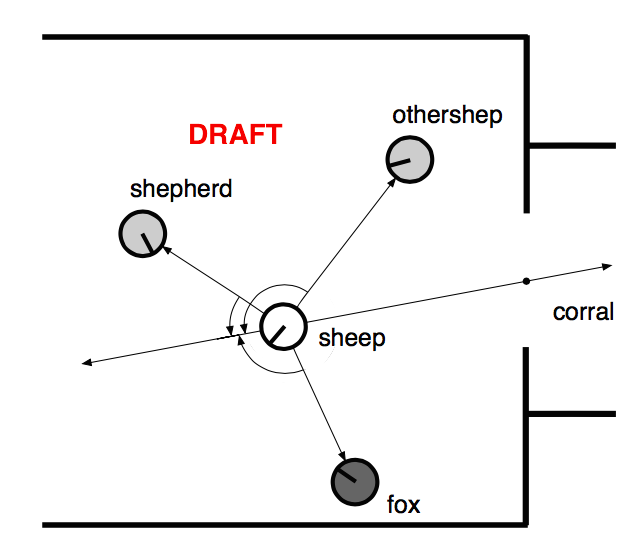
\includegraphics[width=0.8\hsize]{imgs/herding_environment.png}
	\caption{Herding task environment and detail of the positioning coordinates for a group of sheep.}
	\label{fig:task_env}
\end{figure}


\subsection{Neural Networks design}
\label{sec:NN_design}
The controllers for the agents are feedforward neural networks~\cite{bebis1994feed} with one hidden layer.
% Inputs
The inputs for the \glspl{nn} are a fixed \textit{bias} of $1$ and one or more instances of \textit{coordinate pairs} (defined in Section~\ref{sec:herding_task_environment}).
In order to support scenarios with diverse numbers of agents, we design two different NNs: the \textit{single-pair} and the \textit{multi-pair} networks. 
% Single-pair NN
In the case of a \textit{single-pair} network, an agent can only see one other agent so the network consists of two input nodes, one for each item of a \textit{coordinate pair} and its hidden layer has three nodes. 
This network is showed in Figure~\ref{fig:single_pair_topology}.
The input nodes are labelled \textit{opponent} because the input given to the network represents coordinates of an opposing agent.
% Multi-pair NN
Alternatively, to enable an agent to cooperate with its allies, we assign to it a \textit{multi-pair} neural network, with four input nodes for the \textit{coordinate pairs}, and five nodes in its hidden layer.
This \gls{nn} design is shown in Figure~\ref{fig:multi_pair_topology}.
The input nodes are labelled \textit{opponent} and \textit{ally} because the inputs given to the network represent coordinates of one opponent and one ally.

Moreover, for every \glspl{nn} the activation function is a sigmoid function $S(t) = (1 + e^{-t})^{-1}$, centred at $0$. 
The output of the network is a polar \textit{coordinates pair}, namely \textit{target position}, that represents the
location towards which the agent will try to move to in the next time step.
Finally, the output of the \gls{nn} has a range from $(0, 1)$, so in order to convert this into the used positioning system it is translated into a range of $[0, l]$ for target ranges and $[-\pi, \pi]$ for target bearings. 
 
\begin{figure}[t]
	\centering
	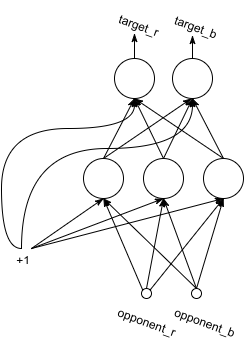
\includegraphics[width=0.5\hsize]{imgs/nn-design_single.png}
	\caption{Single-pair neural network.}
	\label{fig:single_pair_topology}
\end{figure}

\begin{figure}[t]
	\centering
	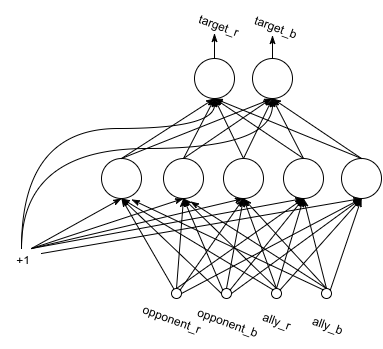
\includegraphics[width=0.8\hsize]{imgs/nn-design_multi.png}
	\caption{Multi-pair neural network.}
	\label{fig:multi_pair_topology}
\end{figure}

\vspace{0.5em}
% Shepherds controllers
\subsubsection{Shepherds controllers}
Shepherds evolve \textit{cooperative} behaviours among themselves to successfully herd sheep.
Therefore, the \textit{competitive} behaviour is against the sheep, who attempts to escape.
In order to pursue cooperation, a shepherd needs information about the other shepherds around. 
However, in order to keep the network complexity low we only provide the controller with information for the closest shepherd. 
Similarly, the competition creates the need for the shepherd to have information about the sheep.
Thus, the inputs for a shepherd controller are: 

\begin{enumerate}
	\item \textit{closestSheep\_r}: Distance from this shepherd to the closest sheep.
	\item \textit{closestSheep\_b}: Bearing between this shepherd and the closest sheep. 
	\item \textit{closestShepherd\_r}: Distance from this shepherd to the closest other shepherd.
	\item \textit{closestShepherd\_b}: Bearing between this shepherd and the closest other shepherd.
\end{enumerate}

We highlight that the third and fourth inputs are not taken into account in scenarios where there is only one shepherd. 

\vspace{0.5em}
% Sheep controllers
\subsubsection{Sheep controllers}
In case of the sheep, competitive and cooperative behaviours are pursued using the same logic as the shepherd's when defining the \gls{nn} inputs. 
This time, in order to avoid the shepherd and be able to escape, sheep have information about the closest shepherd. 
Yet, they have a strong preference to stay in a group and so need information about the closest sheep around them in order to pursue this goal. 
Thus, the inputs for a sheep's controller are:

\begin{enumerate}
	\item \textit{closestShepherd\_r}: Distance from this sheep to the closest shepherd.
	\item \textit{closestShepherd\_b}: Bearing between this sheep and the closest shepherd.
	\item \textit{closestSheep\_r}: Distance from this sheep to the closest other sheep.
	\item \textit{closestSheep\_b}: Bearing between this sheep and the closest other sheep.
\end{enumerate}

Once again, we point out the third and fourth inputs are not taken into account in scenarios where there is only one sheep. 

\subsection{Evolution of controllers}
\label{sec:controllers_evolution}
The algorithm used to evolve the controllers follows the framework of evolution strategies (ES) \cite{back1993overview}. 
We use the ($\mu + \lambda$) strategy, with $\mu = 10$ and $\lambda = 100$~\cite{eiben2003introduction}. 
An ($\mu + \lambda$) ES generates $\lambda$ children from a population of $\mu$ individuals by mutating them; therefore no crossover operator is used.
The $\mu + \lambda$ children are then evaluated and the best $\mu$ individuals among them are selected for the next generation.
The genome is a real-valued vector representing the connection weights of the neural network.
The genome can be of two sizes (depending on the scenario): $17$ for the \textit{simple-pair} network and $37$ for the \textit{multi-pair} network. 
Furthermore, each individual in a population is evaluated with the best individuals from the other populations, following an elitist approach.
Different fitness functions are created for each type of agent, we hereby explain each of them and motivate its design.

\vspace{0.5em}
\subsubsection{Shepherd fitness function}
In order to show the shepherd fitness function, Equation~\eqref{eq:gcDist} introduces the euclidean distance from the sheep center of group mass $gc$ (see Section~\ref{sec:herding_task_environment}) to the corral position $cr$.
Given $t$ as an incremental index of the simulation time steps, it is defined as:
% GROUP CENTER OF MASS DISTANCE
\begin{equation} \label{eq:gcDist}
gcd(t) = \sqrt{(cr_x - gc_x(t))^2 + (cr_y - gc_y(t))^2}
\end{equation}
This metric grows as the group of sheep distance itself from the corral in the attempt to escape.
Furthermore, at every time step a \textit{bonus} is rewarded for corralling a sheep or a \textit{penalty} is deducted for letting a sheep escape. 
Each of these rewards is regulated by the elapsed simulation time, meaning that a bonus/penalty is larger the earlier the rewarded event happens.
% SHEPHERD BONUS
\begin{equation} \label{eq:bonus}
bonus(t) = - l (T - t)
\end{equation}
% SHEPHERD PENALTY
\begin{equation} \label{eq:penalty}
penalty(t) = l (T - t)
\end{equation}
Where $T$ is the number of total steps (1500 in our experiments) and $t$ is the number of elapsed steps the moment the simulation is stopped.
Finally, the fitness for shepherds is defined as the cumulative distance from the sheep center to the corral position~\eqref{eq:gcDist} taking into account bonuses~\eqref{eq:bonus} and penalties~\eqref{eq:penalty}, over every simulation time step:
% SHEPHERD FITNESS
\begin{equation} \label{eq:shep_fitness}
f_{sheph} = \sum_{i=1}^{1500} gcd(i)	+ bonus(i) + penalty(i)
\end{equation}
In order to observe herding behaviour,~\eqref{eq:shep_fitness} has to be minimized.
Note that the fitness is the same among a group of shepherds, since all the components reflect on the group's performance. 
This design choice is motivated by the fact that shepherds must work together to achieve a common goal. 

\vspace{0.5em}
\subsubsection{Sheep fitness function}
The fitness for a sheep is determined by its own distance to the corral. 
% SHEEP DISTANCE
\begin{equation} \label{eq:sheep_dist}
sd(t) = \sqrt{(cr_x - sheep_x(t))^2 + (cr_y - sheep_y(t))^2}
\end{equation}
In scenarios involving more than one sheep, a group component is added to motivate sheep to stay together. 
This is the radius $\rho$ of the group calculated as the distance from the furthest sheep $\alpha$ to the center of mass $gc$ in a specific time step.
% SHEEP RATIO
\begin{equation} \label{eq:sheep_ratio}
\rho(t) = \sqrt{(\alpha_x(t) - gc_x(t))^2 + (\alpha_y - gc_y(t))^2}
\end{equation}
Similarly to the shepherds, bonuses and penalties are given when a sheep escapes or is corralled, accordingly:
% SHEEP BONUS
\begin{equation} \label{eq:sheep_bonus}
f_{sheep}(x) = f_{sheep}(x) + l (T - t)
\end{equation}
% SHEEP PENALTY
\begin{equation} \label{eq:sheep_pen}
f_{sheep}(x) = f_{sheep}(x) - l (T - t)
\end{equation}
Where $T$ is the number of total steps (1500 in our experiments) and $t$ is the number of elapsed steps when the simulation stopped.
Since larger distances but smaller ratios are desired, the fitness function is determined as the individual distance minus the group ratio, added over the simulation time steps. 
% SHEEP FITNESS
\begin{equation} \label{eq:sheep_fitness}
f_{sheep}(x) = \sum_{i=1}^{1500}(sd(i) - {RR} \rho(i))
\end{equation}
where $0 \leq RR \leq 1$ is a constant that controls the weight of the sheep-radius component on the sheep's fitness score.


\subsection{Agents}
\label{sec:agents_design}
% Obstacle avoidance
The output of the \gls{nn} produces a target position for the agents to move towards.
However, both types of agents have an obstacle avoidance mechanism that may override the network's output, hindering an agent's movement when necessary.
To achieve this, each agent is provided with a \textit{radius} which allows to push other agents with a smaller radius.
Obstacles entering this radius hinder the agent from moving in this direction and will reposition the agent preventing overlap between object and radius.
We assign a greater radius to the shepherd than to the sheep, by doing so we allow the shepherd to push, and thus herd, the sheep towards the corral.

% Interpreting the Neural Network output
Since the output of the network is represented as polar coordinates centred with the polar axis passing through the nearest opponent, they are translated into Cartesian coordinates within the pasture to calculate the agents target position.
All agents have the same maximum speed and mass, so their simulated physical characteristics are the same.
Both maximum speed and mass have a value of $1$ simulated units.



\section{Experimental results}
\label{sec:experiment}
In order to answer the research questions listed in {Section~\ref{sec:researchQuestions}} and test its corresponding hypothesis in {Section~\ref{sec:hypothesis}}, we execute the co-evolutionary algorithm in the different scenarios for $100$ generations. 
We run the entire evolutionary process for $40$ times and perform statistical analysis to get $95\%$ confidence intervals and $t$-test.

\subsection{Implementation}
\label{sec:implementation}
The project is coded in Java and has a GUI to launch the different experiments, replay the best individuals for each generation and plot statistics.
The evolutionary algorithm is implemented through the use of \textit{ECJ} \cite{luke2006ecj}: an easy to use evolutionary computation research framework with out-of-the-box algorithms and tools that enabled us to implement our co-evolutionary ES.
To realise the simulation environment and its agents, we use \textit{MASON} \cite{luke2005mason}, developed at the George Mason University's ECLab Evolutionary Computation Laboratory as a sister project of ECJ.
Moreover, we use \textit{neuroph} \footnote{http://neuroph.sourceforge.net/} to create and handle the neural networks.

Because with a co-evolutionary setting ECJ can only do maximization problems, the shepherd fitness score is negated in the implementation, that is:
$$ f_{sheph}(x) = -f_{sheph}(x) $$
In our experiments we give a value of $0.8$ to the constant $RR$ of equation \eqref{eq:sheep_fitness}, reducing the weight given to the flocking behaviour produced by \eqref{eq:sheep_ratio}.

Similarly to \cite{potter2001heterogeneity}, a simulation consists of 2.5 simulated minutes and the agents refresh their target position every 10Hz.
This is equivalent to $1500$ simulation steps in which the agents refresh their target every step.
To do so, an agent firstly acquires its inputs and then propagates them through its neural network computing a new target position that the simulation environment will translate in forces to be applied to the agent's virtual body.


\vspace{0.5em}
\subsubsection{Environment and Agents}
The size of the pasture is fixed across all the experiments at $l = 37$ simulated units.
As already stated in Section \ref{sec:agents_design}, the shepherd is equipped with a greater radius than the sheep's.
This is to allow them to effectively herd the sheep by rimming and pushing it towards the corral.
Therefore we assign a radius of $3$ and $2$ simulation units to the shepherd and to the sheep respectively.
The pasture is closed on the top and bottom sides, with the corral positioned on the right side, opposite to an open side that enables the sheep to escape.
The initial positions of the agents inside the pasture are shown in Figure \ref{fig:simulation_screenshot} for a full \textit{three vs. three} experiment.
The initial locations values used in the experiments are:
\begin{align}
sheph_x &= \frac{l}{2} - 6 \\
sheph_y(i) &= \frac{l}{2} + \begin{cases} 0 & \text{if } i=1 \\ -6 & \text{if } i=2 \\ +6 & \text{if } i=3 \end{cases} \\
sheep_x &= \frac{l}{2} + 6 \\
sheep_y(i) &= \frac{l}{2} + \begin{cases} 0 & \text{if } i=1 \\ -4 & \text{if } i=2 \\ +4 & \text{if } i=3 \end{cases}
\end{align}

\begin{figure}[t]
	\centering
	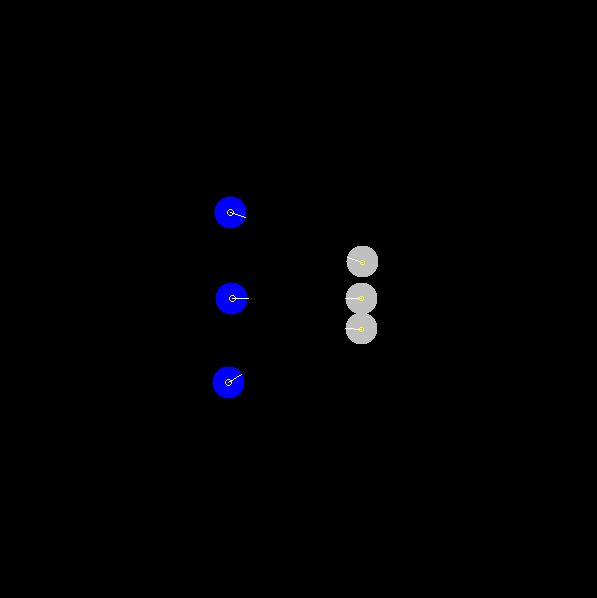
\includegraphics[width=0.8\hsize]{imgs/pasture.png}
	\caption{Screenshot of the simulation with the shepherds (blue ones) and the sheep (gray ones), almost at the starting locations.}
	\label{fig:simulation_screenshot}
\end{figure}


\subsubsection{Evolution}
In order to calculate the fitness for an individual, all controllers are evaluated through 10 trials of the task and the average is taken as fitness.
Every trial runs for a maximum of $1500$ time steps. 
In cases where there is more than one sheep, a complex network is assigned to all sheep. 
The simulation ends before the time elapses as soon as one sheep is corralled or escapes. 
The reason for leaving one sheep left in the pasture when ending the simulation is that the number of inputs for the sheep controllers is fixed before the beginning of a trial, and having no other sheep left would lead to null inputs and misbehaviour. 
In cases where there is only one sheep, a simple controller is assigned. 
Thus, the sheep must either be corralled or has to escape in order for the simulation to stop before the time expires.

In homogeneous set-ups we evolve one controller per type of agent, meaning we have two subpopulations, one for shepherds and one for sheep, co-evolving. 
However, to create heterogeneity a population per agent is created. 
For example, in a scenario with two shepherds and one sheep, there is a total of three subpopulations, two of them cooperating among each other and competing with the third one.  



\subsection{Performance details}
\label{sec:experiments_performances}
In this section we present the results of the experiments run using the implementation detailed in Section~\ref{sec:implementation}.
% Homo vs Hetero experiment
\vspace{0.5em}
\subsubsection{Homogeneity vs Heterogeneity}
We first consider two experiments that relate to the first research question: \textit{How do homogeneous and heterogeneous shepherd controllers compare in a competitive co-evolved herding task?}. 
Here, the independent variable is the controller type (homogeneous or heterogeneous). The dependent variable is the fitness score for the best fitted shepherds so far. 
Figure~\ref{fig:2v1_homo_vs_hetero} reports the shepherds' fitness score on a scenario with two shepherds and one sheep, while Figure~\ref{fig:3v1_homo_vs_hetero} reports the score on a scenario with three shepherds and one sheep.
The graphs represent the mean fitness of the best individual seen so far, averaged over 40 trials, with 95-percent confidence intervals.
Moreover, we perform \textit{t}-test on the means of the homogeneous and heterogeneous trials. The test  produced a \textit{p}-value $\ll0.5$ for both cases.
Thus, supported by the significant difference between the homogeneous and heterogeneous cases, we reject the corresponding null hypothesis (see Section~\ref{sec:hypothesis}).
Additionally, both graphs show that homogeneous controllers outperform heterogeneous controllers. Thus, we reject hypothesis $H_1$ as well.

\begin{figure}[ht]
	\centering
	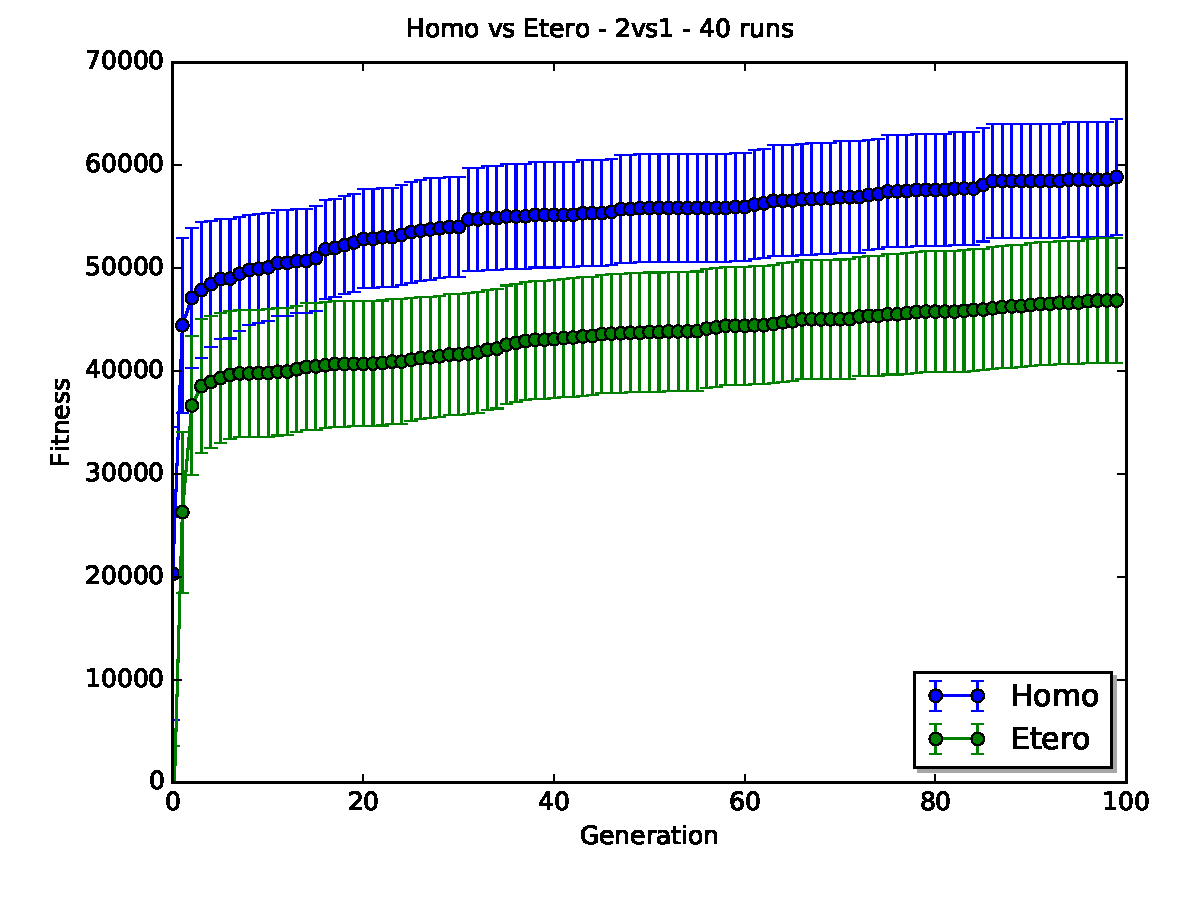
\includegraphics[width=1\hsize]{imgs/homo2v1-hetero2v1-bestSoFar.pdf}
	\caption{Best individuals fitness in scenario with two shepherds and one sheep. Both homogeneous and heterogeneous settings are shown}
	\label{fig:2v1_homo_vs_hetero}
\end{figure}

\begin{figure}[ht]
	\centering
	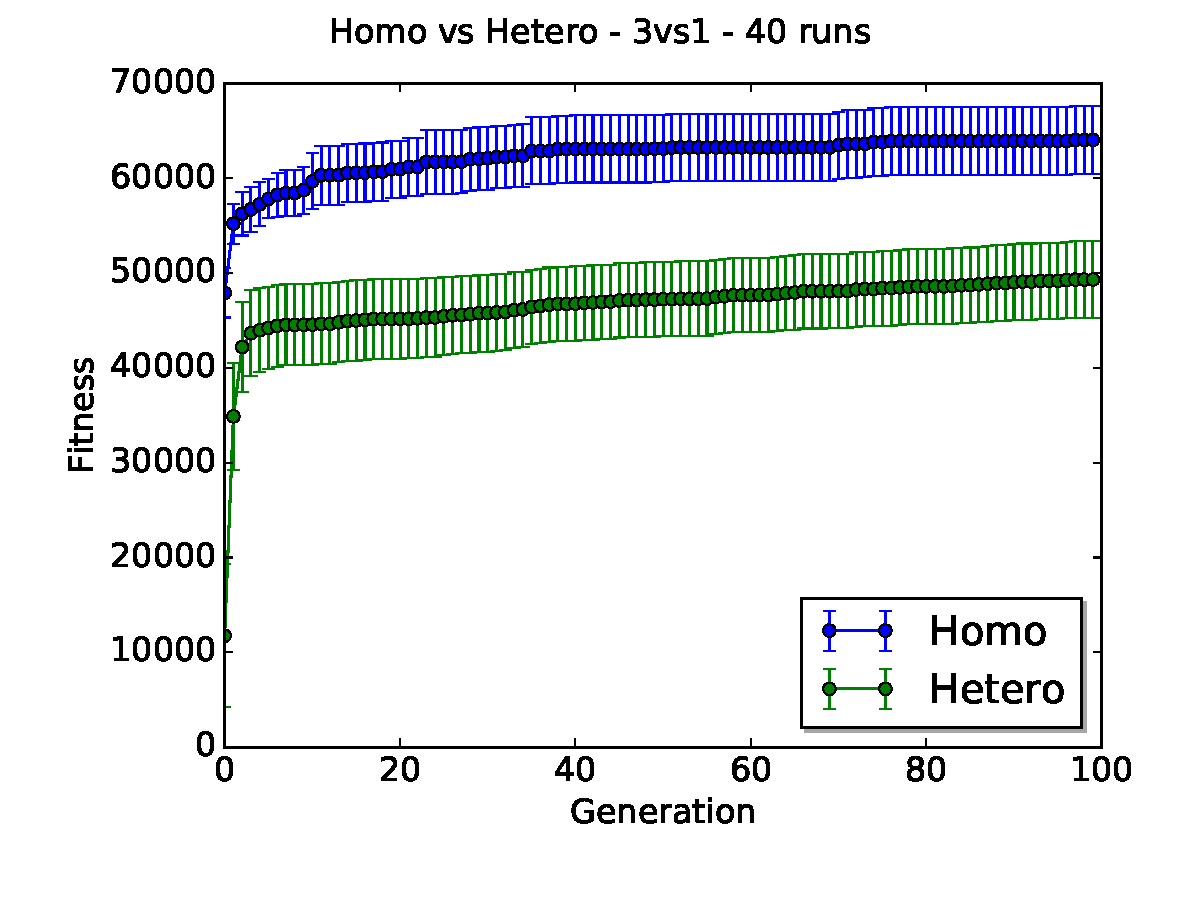
\includegraphics[width=1\hsize]{imgs/homo3v1-hetero3v1-bestSoFar.pdf}
	\caption{Best individuals fitness in scenario with three shepherds and one sheep. Both homogeneous and heterogeneous settings are shown}
	\label{fig:3v1_homo_vs_hetero}
\end{figure}


\begin{figure}[ht]
	\centering
	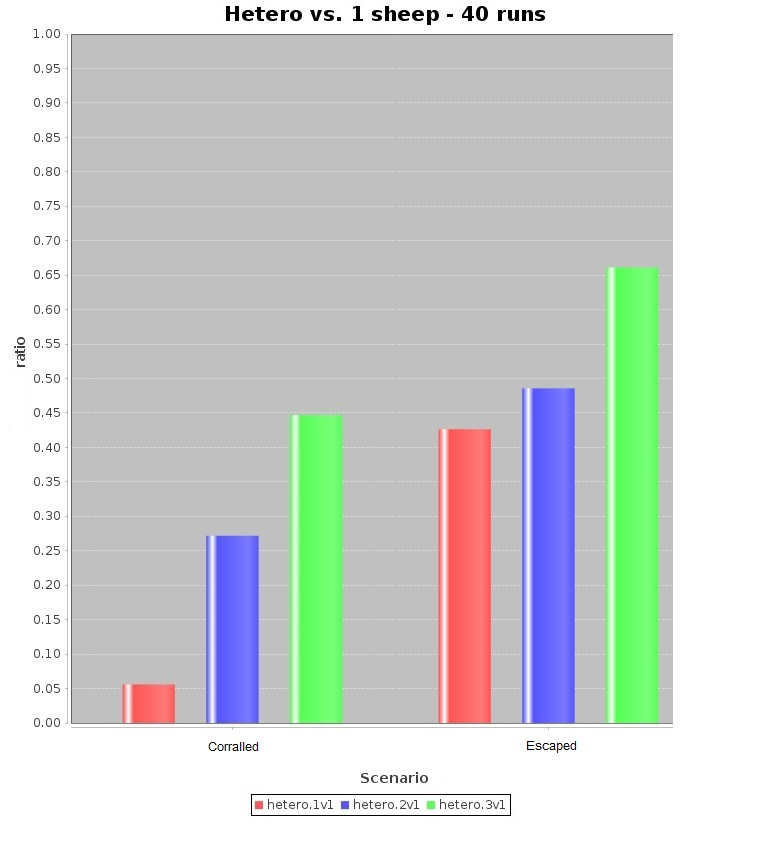
\includegraphics[width=3in]{imgs/hetero_1v1-hetero_2v1-hetero_3v1-ratio-bar.jpg}
	\caption{Bar chart for corralled and escaped ratios in heterogeneous setting. Shows one, two and three shepherds herding one sheep.}
	\label{fig:ratios_oneSheep}
\end{figure}

\begin{figure}[ht]
	\centering
	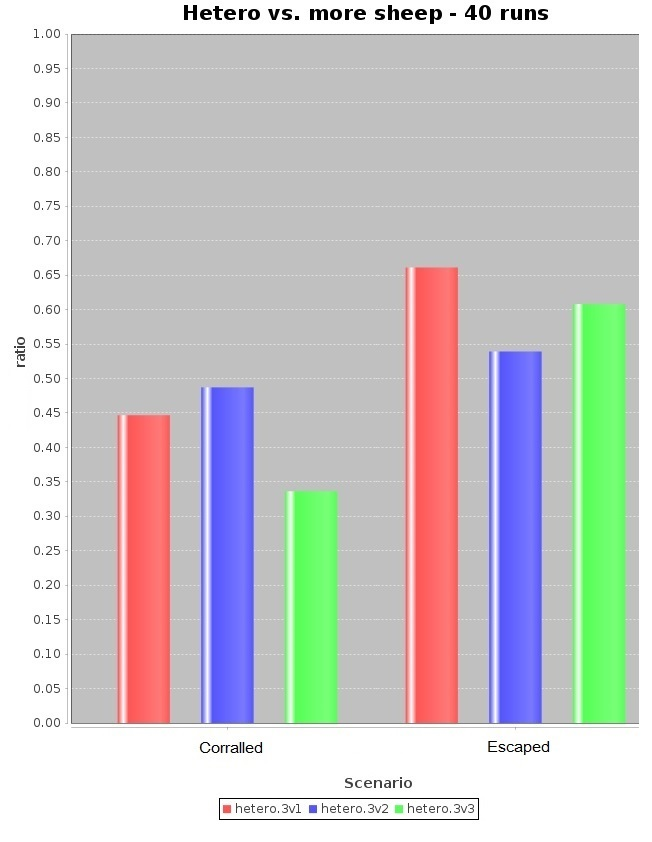
\includegraphics[width=3in]{imgs/hetero_3v1-hetero_3v2-hetero_3v3-ratio-bar.jpg}
	\caption{Bar chart for corralled and escaped ratios in heterogeneous setting. Shows three shepherd herding one, two and three sheep.}
	\label{fig:ratios_threeShepherd}
\end{figure}


\begin{table*}[t]
	\centering
	\begin{tabularx}{6in}{| L{0.4} | L{0.4} | C{1} C{1} C{1} |}
		\hline
		\textit{\textbf{Shepherds}} & \textit{\textbf{Sheep}} & \multicolumn{3}{c|}{\textit{\textbf{Fitness}}} \\
		& & \textit{Mean} & \textit{Minimum} & \textit{Maximum} \\
		\hline
		1 & 1 & 2 $\pm$ 0.1 & 0 & 10 \\
		%\hline
		2 & 1 & 2 $\pm$ 0.1 & 0 & 10 \\
		\hline
		3 & 1 & 2 $\pm$ 0.1 & 0 & 10 \\
		\hline
		3 & 2 & 2 $\pm$ 0.1 & 0 & 10 \\
		%\hline
		3 & 3 & 2 $\pm$ 0.1 & 0 & 10 \\
		\hline
	\end{tabularx}
	\caption{\textbf{TODO} Comparison of the mean fitness of the heterogeneous shepherds vs. homogeneous sheep over 40 runs.}
	\label{tab:1}
\end{table*}

% Task complexity
\vspace{0.5em}
\subsubsection{Task complexity}
Here we consider three experiments that relate to the second research question: \textit{How does varying task complexity (by moduling the sheep to shepherds ratio) affect the effectiveness of herding?}. 
This time, the independent variable is the task complexity, previously defined as the sheep to shepherd ratios $\phi = S / D$. First we investigate $H_2$ by keeping a fixed number of sheep, and increasing the number of shepherd herding it thus decreasing the task complexity. The experiments consider the following scenarios:
\begin{itemize}
	\item one shepherd herding one sheep: $\phi = 1$
	\item two shepherds herding one sheep: $\phi = 0.5$
	\item three shepherds herding one sheep: $\phi = 0.33$
\end{itemize}	
Subsequently, we investigate $H_3$ by keeping a fixed number of shepherd, and increasing the number of sheep being herd thus increasing the task complexity. These experiments consider the following scenarios:
\begin{itemize}
	\item three shepherd herding one sheep: $\phi = 0.33$
	\item three shepherd herding two sheep: $\phi = 0.66$
	\item three shepherd herding three sheep: $\phi = 1$
\end{itemize}
The dependent variables are the corralled and escaped sheep ratios the best fitted individuals achieved in the last generation.
Figure~\ref{fig:ratios_oneSheep} shows the corralled and escaped ratios for different number of shepherd herding one sheep. Figure~\ref{fig:ratios_threeShepherd} shows the corralled and escaped ratios for three shepherd herding different number of sheep. 
%TODO confidence intervals. Mention in text only. 
The chart in Figure ~\ref{fig:ratios_oneSheep} provides supporting evidence for $H_2$. Adding a second shepherd to the task improves the corralled score by 400\% while adding a third shepherd has an increase of 800\% compared to a simple case with just one shepherd. 
However, we notice that the ratio for escaped cases increases as well, meaning that overall the tied cases (cases where the simulations run till the end without shepherds of sheep being successful) are decreased. 
Relating this to competitive co-evolution, it is reasonable to think that increasing the number of shepherds encourages both shepherds and sheep to pursue their goals more aggressively.
Contrarily, the chart in Figure ~\ref{fig:ratios_threeShepherd} does not provide supporting evidence for $H_3$ since adding sheep to the task does not have an evident effect. Therefore, we accept the corresponding null hypothesis (see Section~\ref{sec:hypothesis}). 

\section{Conclusion}
\label{sec:conclusion}
Given the above information, we conclude that shepherds benefit from homogeneous controllers in a competitive co-evolved herding task. 
Given heterogeneous controllers and a fixed number of sheep to be herded, adding shepherds encourages more aggressive behaviours. More shepherds cooperate to corral more sheep, but the effectiveness in herding leads to sheep becoming better at escaping. 
Given heterogeneous controllers and a fixed number of shepherds, adding more sheep to the task has no direct influence on the effectiveness in herding.
The last two findings lead to the conclusion that simply changing the task complexity does not have a conclusive effect on the effectiveness of herding. The number of each type of agent matters, and some specific conditions make co-evolution more competitive.


\printbibliography

\end{document}

